\documentclass[12pt,letterpaper]{article}
\usepackage[utf8]{inputenc}
\usepackage[spanish,es-tabla]{babel}
\decimalpoint
\let\cleardoublepage\clearpage
\usepackage[bitstream-charter]{mathdesign} 
\usepackage[T1]{fontenc}
\newcommand{\selectSans}{\usefont{T1}{qhv}{m}{n}\selectfont} % sans-serif TeX Gyre Heros font
\usepackage{amsmath}
\usepackage{amsfonts}
\usepackage{amssymb}
% \usepackage[T1]{fontspec}
\usepackage{color}
\usepackage{graphicx}
\usepackage{makeidx}
\makeindex
\usepackage{anysize}
\usepackage{anyfontsize}
\usepackage{pdfpages}
\usepackage[x11names,table]{xcolor}
\usepackage{tikz}
\usepackage{tcolorbox}
\tcbuselibrary{skins,breakable,listings,theorems}
\usepackage[hidelinks]{hyperref}
\usepackage[labelfont=bf]{caption}
\captionsetup[table]{labelsep=space}
\captionsetup[figure]{labelsep=space}
\usepackage{listings}
\usepackage{array,ragged2e}
\usepackage{multirow}
\usepackage[left=2cm,top=2cm,right=2cm,bottom=2cm]{geometry}
\setlength{\parindent}{0cm}
% \usepackage[printwatermark]{xwatermark}
% \newwatermark[allpages,color=gray!10,angle=45,scale=3,xpos=0,ypos=0]{Borrador}

\tcbset{colback=green!5!white, colframe=gray!10!black, coltitle=green!20!black, 
fonttitle=\bfseries, colbacktitle=white, coltext=gray!30!black}
\addto\captionsspanish{
  \renewcommand{\figurename}{{\bf Figura}}% 
}
\addto\captionsspanish{
  \renewcommand{\chaptername}{{\bf}}% 
}

\usepackage{epigraph}
\usepackage{fontawesome}
\usepackage[Bjornstrup]{fncychap}

% \renewcommand{\familydefault}{\sfdefault}

% Colores
\definecolor{verdep}{RGB}{166,206,58}
\definecolor{ccap}{RGB}{10,10,50}
\definecolor{csec}{RGB}{50,50,100}
\definecolor{csubsec}{RGB}{80,80,120}
\definecolor{header_table_color}{RGB}{200,255,180}
\definecolor{info_color}{RGB}{100,100,200}
\definecolor{csol}{rgb}{0.2,0.8,0.1}
\definecolor{backcode}{rgb}{0.98,0.98,0.99}
\definecolor{crule}{rgb}{0.9,0.9,0.9}
\definecolor{dkgreen}{rgb}{0,0.6,0}
\definecolor{gray}{rgb}{0.5,0.5,0.5}
\definecolor{mauve}{rgb}{0.58,0,0.82}


\newtcolorbox{ejemplo}[2][]
{
  breakable,
  colframe = gray!50,
  colback  = gray!0,
  coltitle = gray!20!black,
  title    =  \faEdit \hspace{5 mm} #2,
}

\newtcolorbox{informacion}[2][]
{
  breakable,
  colframe = blue!5!white,
  colback  = blue!5!white,
  coltitle = blue!80!black,
  title    = \faInfo \hspace{5 mm} #2,
}

\newtcolorbox{recomendacion}[2][]
{
  breakable,
  colframe = green!25,
  colback  = green!10,
  coltitle = green!20!black,
  title    = #2,
}

 \newcommand{\ccol}{>{\centering\tt\arraybackslash}}

% Nuevos comandos

\usepackage{titlesec}%--
% \newcommand{\hsp}{\hspace{5pt}}
% \titleformat{\chapter}[hang]{\huge\bfseries\color{ccap}}
% {\color{verdep}{\vrule height 2.5cm width 1mm}\hsp{\fontsize{100}{5}\selectfont\thechapter}\hsp%
% {\vrule height 2.5cm width 1mm}\hsp{\fontsize{30}{5}\selectfont}}{5pt}{\huge\bfseries}

\titleformat{\section}[hang]{\normalfont\color{csec}}%
{\filright\large\enspace\thesection\enspace}%
{8pt}{\Large\bfseries\filright}%

\titleformat{\subsection}[hang]{\normalfont\color{csec}}%
{\filright\large\enspace\thesubsection\enspace}%
{8pt}{\large\bfseries\filright}%

% Code
\lstnewenvironment{matlab}{\lstset{frame=single,
  frameround=tttt,
  backgroundcolor=\color{backcode},
  rulecolor=\color{crule},
  language=matlab,
  aboveskip=5mm,
  belowskip=5mm,
  showstringspaces=false,
  columns=flexible,
  basicstyle={\small\ttfamily},
  numbers=none,
  numberstyle=\tiny\color{gray},
  keywordstyle=\color{blue},
  commentstyle=\color{dkgreen},
  stringstyle=\color{mauve},
  breaklines=true,
  breakatwhitespace=true,
  tabsize=4,
  extendedchars=true,
  inputencoding=utf8,
  literate=%
  {°}{{\,\,$^\circ$\,\,}}1
  {á}{{\'a}}1
  {é}{{\'e}}1
  {í}{{\'i}}1
  {ó}{{\'o}}1
  {ú}{{\'u}}1
  {Á}{{\'A}}1
  {É}{{\'E}}1
  {Í}{{\'I}}1
  {Ó}{{\'O}}1
  {Ú}{{\'U}}1
}}{}


% \author{Pedro Jorge De Los Santos}
\title{
{\Large Mecánica de Materiales} \\
{\large Problemario Unidad I} \\
}

% =================================================================
% =================================================================
%                              CONTENIDO
% =================================================================
% =================================================================

\begin{document}
\maketitle

\begin{ejemplo}{Ejercicio 1}

Una barra horizontal CDB que tiene una longitud de 2.2 m está soportada y cargada como se muestra 
en la figura. El elemento vertical AB tiene un área de sección transversal de 540 $\text{mm}^2$. 
Calcule la magnitud de la fuerza P que produce un esfuerzo normal de 50 MPa en el elemento AB.

\begin{center}
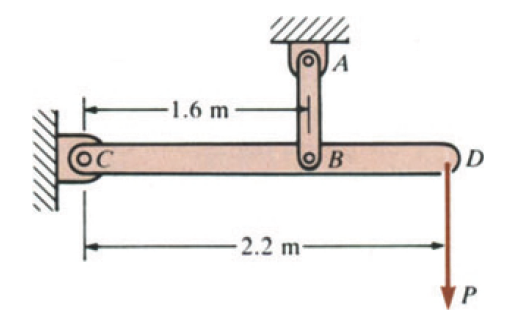
\includegraphics[width=0.45\textwidth]{img/p01.PNG}
\end{center}

\end{ejemplo}


\begin{ejemplo}{Ejercicio 2}

Una barra de acero de 1 m de longitud y 12 mm de diámetro soporta una carga a tensión de 13.3 kN. La barra 
incrementa su longitud en 0.5 mm cuando la carga es aplicada. Determine el esfuerzo normal y la deformación.

\begin{center}
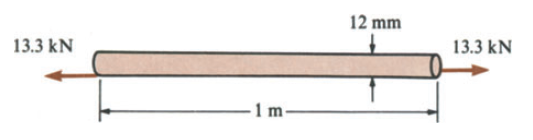
\includegraphics[width=0.55\textwidth]{img/p02.PNG}
\end{center}

\end{ejemplo}


\begin{ejemplo}{Ejercicio 3}

Se realiza un ensayo de tensión a una probeta de latón de 10 mm de diámetro usando una longitud calibrada de 50 mm. 
Cuando la fuerza tensionante P alcanza un valor de 25 kN, la distancia entre las marcas se ha incrementado 
en 0.152 mm. (a) ¿Cuál es el módulo de elasticidad del latón? (b) ¿Cuál es el decremento $\Delta d$ en el 
diámetro de la barra?

\begin{center}
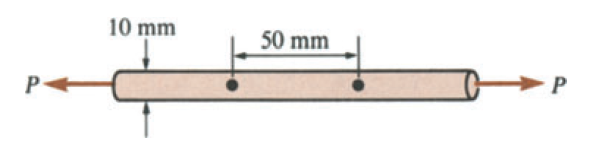
\includegraphics[width=0.55\textwidth]{img/p03.PNG}
\end{center}

\end{ejemplo}


\begin{ejemplo}{Ejercicio 4}

La fuerza vertical P actuando en la rueda de una grúa móvil es de 53 kN. ¿Cuál es el esfuerzo cortante 
promedio $\tau$ en el eje de 38 mm de diámetro?.

\begin{center}
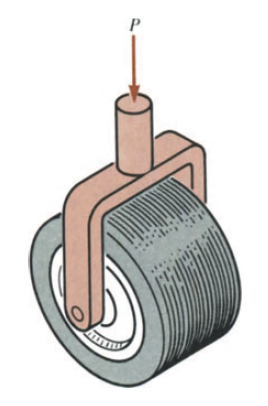
\includegraphics[width=0.2\textwidth]{img/p04.PNG}
\end{center}

\end{ejemplo}


\begin{ejemplo}{Ejercicio 5}

La junta de traslape mostrada en la figura está unida por cuatro remaches de 3/4 in de diámetro. Calcule 
la máxima fuerza P que puede ser aplicada si el esfuerzo de trabajo es de 14 ksi a cortante en el remache 
y de 18 ksi para los apoyos en la placa. Asuma que la fuerza aplicada está distribuida uniformemente en 
los cuatro remaches, y desprecie la fricción entre las placas.

\begin{center}
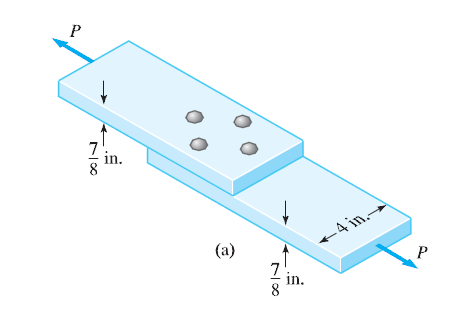
\includegraphics[width=0.5\textwidth]{img/p05.PNG}
\end{center}

\end{ejemplo}


\begin{ejemplo}{Ejercicio 6}

La barra de caucho de 50 mm de diámetro es colocada dentro de un agujero con paredes rígidas y lubricadas. 
No hay claros entre la barra y los lados del agujero. Calcule el cambio en la longitud de la barra cuando 
una carga de 8 kN es aplicada. Use $E=40 \text{ MPa}$ y $\nu = 0.45$ para el caucho.

\begin{center}
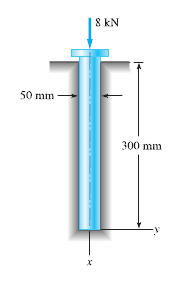
\includegraphics[width=0.32\textwidth]{img/p06.PNG}
\end{center}

\end{ejemplo}


\begin{ejemplo}{Ejercicio 7}

Tres tornillos son utilizados para fijar la placa de acero a la viga de madera 
mostrada en la figura. Sabiendo que la placa soporta 110 kN de carga y que el 
esfuerzo cortante de trabajo en los tornillos no debe ser de mayor de 80 MPa, 
calcule el diámetro mínimo de los tornillos a utilizar.

\begin{center}
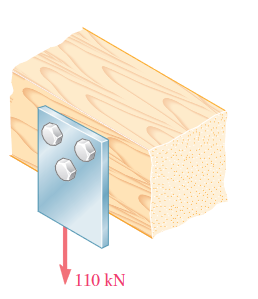
\includegraphics[width=0.32\textwidth]{img/p07.PNG}
\end{center}

\end{ejemplo}


\begin{ejemplo}{Ejercicio 8}

Dos elementos de madera de sección transversal rectangular están unidos mediante pegamento como se muestra en la figura. Sabiendo que 
P = 11 kN, calcule el esfuerzo normal y cortante en el pegamento.

\begin{center}
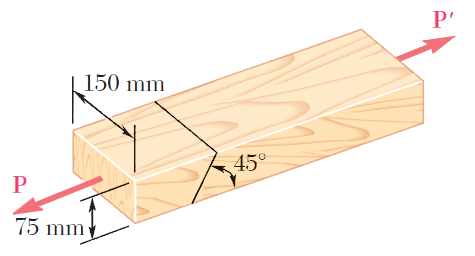
\includegraphics[width=0.4\textwidth]{img/p08.PNG}
\end{center}

\end{ejemplo}


\begin{ejemplo}{Ejercicio 9}

El eslabón AC tiene una sección transversal rectangular de 1/16 in. de espesor y 1/4 in. de ancho. Calcule 
el esfuerzo normal en la porción central del eslabón.

\begin{center}
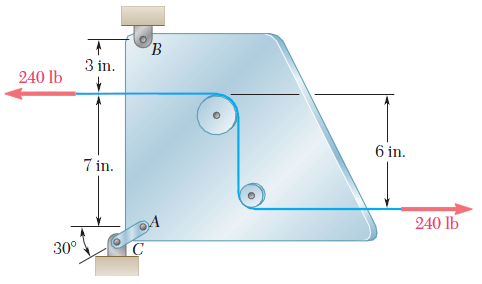
\includegraphics[width=0.55\textwidth]{img/p09.PNG}
\end{center}

\end{ejemplo}


\begin{ejemplo}{Ejercicio 10}

Cuando la fuerza P alcanza 8 kN, el especimen de madera falla por cortante a lo largo de la superficie indicada 
por la línea punteada. Calcule el esfuerzo cortante promedio a lo largo de esa superficie al momento de la falla.

\begin{center}
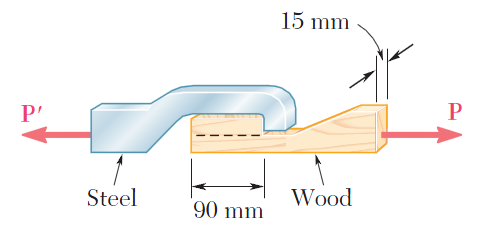
\includegraphics[width=0.55\textwidth]{img/p10.PNG}
\end{center}

\end{ejemplo}




\end{document}